%%
%% This is file `sample-acmsmall.tex',
%% generated with the docstrip utility.
%%
%% The original source files were:
%%
%% samples.dtx  (with options: `acmsmall')
%% 
%% IMPORTANT NOTICE:
%% 
%% For the copyright see the source file.
%% 
%% Any modified versions of this file must be renamed
%% with new filenames distinct from sample-acmsmall.tex.
%% 
%% For distribution of the original source see the terms
%% for copying and modification in the file samples.dtx.
%% 
%% This generated file may be distributed as long as the
%% original source files, as listed above, are part of the
%% same distribution. (The sources need not necessarily be
%% in the same archive or directory.)
%%
%% The first command in your LaTeX source must be the \documentclass command.
 \documentclass[acmsmall]{acmart}
\usepackage{listings}
\lstset{
	language=bash,
	basicstyle=\ttfamily
}
%%
%% \BibTeX command to typeset BibTeX logo in the docs
%%\AtBeginDocument{%
 %% \providecommand\BibTeX{{%
  %%  \normalfont B\kern-0.5em{\scshape i\kern-0.25em b}\kern-0.8em\TeX}}}

%% Rights management information.  This information is sent to you
%% when you complete the rights form.  These commands have SAMPLE
%% values in them; it is your responsibility as an author to replace
%% the commands and values with those provided to you when you
%% complete the rights form.



%%
%% These commands are for a JOURNAL article.
%% \acmJournal{JACM}
%% \acmVolume{37}
%% \acmNumber{4}
%% \acmArticle{111}

%%
%% Submission ID.
%% Use this when submitting an article to a sponsored event. You'll
%% receive a unique submission ID from the organizers
%% of the event, and this ID should be used as the parameter to this command.
%%\acmSubmissionID{123-A56-BU3}

%%
%% The majority of ACM publications use numbered citations and
%% references.  The command \citestyle{authoryear} switches to the
%% "author year" style.
%%
%% If you are preparing content for an event
%% sponsored by ACM SIGGRAPH, you must use the "author year" style of
%% citations and references.
%% Uncommenting
%% the next command will enable that style.
%%\citestyle{acmauthoryear}

%%
%% end of the preamble, start of the body of the document source.
\begin{document}

%%
%% The "title" command has an optional parameter,
%% allowing the author to define a "short title" to be used in page headers.
\title{Progetto 2 [SABD]}

%%
%% The "author" command and its associated commands are used to define
%% the authors and their affiliations.
%% Of note is the shared affiliation of the first two authors, and the
%% "authornote" and "authornotemark" commands
%% used to denote shared contribution to the research.
\author{Damiano Nardi}

\email{damiano6276@gmail.com}
\affiliation{%
 \institution{TorVergata, Corso Di Informatica}
 }

%%
%% By default, the full list of authors will be used in the page
%% headers. Often, this list is too long, and will overlap
%% other information printed in the page headers. This command allows
%% the author to define a more concise list
%% of authors' names for this purpose.

%%
%% The abstract is a short summary of the work to be presented in the

%\begin{abstract}

%\end{abstract}
%% article.

%%
%% The code below is generated by the tool at %%http://dl.acm.org/ccs.cfm.
%% Please copy and paste the code instead of the example below.
%%



%%
%% Keywords. The author(s) should pick words that accurately describe
%% the work being presented. Separate the keywords with commas.



%%
%% This command processes the author and affiliation and title
%% information and builds the first part of the formatted document.dsd
 \maketitle{} 

\section{Introduzione}
In questa relazione si descriverà il lavoro svolto che consiste nella realizzazione delle query(1,2) 


\section{Processamento Delle Query}
Per processare le query 1 e 2 è stato usato il framework apache flink usando le api java, inoltre per confrontare flink con kafka streams è stata fatta la anche query 1 usando kafka streams.
Si è utilizzata una macchina virtuale con Ubuntu 20.04 con allocatevi 4 core della cpu (i7-8750H) e 8gb di ram (ddr4 2400 MHz).

\subsection{Stremming del dataset}
Il dataset viene letto e inviato riga per riga a una topica kafka che viene poi consumata da apache flink o da kafka streams.

\subsection{Query1}
\begin{quote}
Calcolare il ritardo medio degli autobus per quartiere nelle ultime 24 ore (di event time), 7 giorni (di
event time) e 1 mese (di event time). L’output della query ha il seguente schema: ts, boro-x, avg-x, ..., boro-z, avg-z
\end{quote}

Lo stream del dataset viene letto da una topica kafka la prima operazione fatta 
è una 
\subsubsection{flatMap} 
In questa flatMap viene processata la singola ringa del dataset andando a mettere come chiave il campo Boro (il quartiere) e come valore un ogetto con questi campi: OccurredOn (data del ritardo), HowLongelayed (ritardo in minuti ) e altri campi meno importanti;
le righe del dataset che non hanno il campo HowLongDelayed o lo hanno in un formato non previsto vengono ignorate.
\subsubsection{EventTime e TumblingEventTimeWindows}
A questo punto flink estrare l'event time dai dati processati della flatMap e 
subito dopo crea una TumblingWindows della durata preimpostata tra 1,7,30 giorni

\subsubsection{Reduce}
Facciamo una reduce (abbiamo che chiave Boro), essenzialmente andiamo a sommare i ritardi di un quartiere (nella stessa finestra) 
teniamo anche in considerazione la "somma" delle reduce fatte e la data più vecchia in ogni reduce.

\subsubsection{Map}
In questa Map andiamo a calcolare la media dei ritardi sommati per ogni quartiere nella precedente reduce

\subsubsection{TumblingEventTimeWindows}
specifichiamo ancora la finestra temporale

\subsubsection{Apply}
In fine vengono raggruppati tutti i dati nella stessa finestra temporale e viene formattato l'output come richiesto dalle specifiche.
\subsubsection{addSink}
Infine viene aggiunto un sink che manda lo stream processato a una topica kafka

\subsection{Query 1 kafka streams}
La query 1 è stata fatta anche su kafka streams le operazioni fatte sono più o meno le stesse, cambia la sintassi, quindi per evitare ridondanza non verranno riportate.


\subsection{Query2}
\begin{quote}
Fornire la classifica delle tre cause di disservizio piu frequenti (ad esempio, Heavy Traffic, Mechanical `
Problem, Flat Tire) nelle due fasce orarie di servizio 5:00-11:59 e 12:00-19:00. Le tre cause sono ordinate dalla piu frequente alla meno frequente. L’output della query ha il seguente schema:
ts, slot-a, rank-a, slot-p, rank-p .\end{quote}

Lo stream del dataset viene letto da una topica kafka la prima operazione fatta 
è una 

\subsubsection{flatMap}
In questa flatMap viene processata la singola riga del dataset andando a mettere come chiave il campo Reason con il prefisso "fascia5-11" o "fascia12-19" scelto in base al campo OccuredOn mentre come valore un ogetto con i seguenti attributi
OccurredOn,Reason,rank(intero inizialmente pari a 1 ), list(inizialmente vuota).


\subsubsection{EventTime e TumblingEventTimeWindows}
A questo punto flink estrare l'event time dai dati processati della flatMap e 
subito dopo crea una TumblingWindows della durata preimpostata tra 1 o 7 giorni


\subsubsection{Reduce}
In questa reduce vengono sommati i campi rank e viene presa la data (OccurredOn) minima tra le varie operazioni di reduce 


\subsubsection{Map}
Viene messa la tupla (Reason,rank) dentro la lista e mettiamo come chiave "fascia5-11" o "fascia12-19"

\subsubsection{TumblingEventTimeWindows}
specifichiamo ancora la finestra temporale

\subsubsection{Reduce}
In questa reduce viene fatto il l'unione del campo lista (che avevamo iniziato a popolare nella map precedente) per le due fascie "fascia5-11", "fascia12-19"

\subsubsection{Map}
Adesso prendiamo la dal campo list le 3 Reason che hanno il rank più alto

\subsubsection{TumblingEventTimeWindows}
Specifichiamo ancora la finestra temporale

\subsubsection{Reduce e Map}
In fine facciamo una Reduce e una Map ai fine formattare l'output come richiesto dalle specifiche
\subsubsection{addSink}
Viene aggiunto un sink che manda lo stream processato a una topica kafka


\section{Tempi}

Sono stati misurati i tempi di latenza e throughput di messaggi al secondo,
In questo paragrafo descriveremo come sono stati calcolati 


\subsection{Producer}
Come accennato prima abbiamo un producer che legge il dataset riga per riga  e li passa a una topica kafka durante questa operazione appena prima di inserire la riga sulla topica viene aggiunto a inizio riga il timestamp corrente, il producer invia i dati alla topica alla massima velocità possibile.


\subsection{2 tipi di latenza}
Quando viene fatta una reduce andiamo ad unificare più righe del dataset che sono state inserite nella topica a tempi di processamento diversi, durante queste operazioni viene tenuta traccia del tempo di processamento più vecchio e più nuovo, quindi ogni output prodotto da flink e da kafka conterrà 3 tempi:
event time,processing time riga più vecchia,processing time riga più nuova.
Abbiamo la latenza del record più vecchio e la latenza del record più nuovo
per ogni output da flink/kafka

\subsection{Consumer}
Il consumer non fa altro che leggere da una topica kafka (output di flink o kafka streams) registra il timestamp corrente ad ogni record prelevato da quest'ultima e calcola i due tempi di latenza in secondi andando a fare la differenza tra quello corrente e quelli presenti nell'output,

\subsection{throughput}
Per misurare il throughput ho utilizzato questo comando di kafka streams
\begin{lstlisting}[language=bash]
$ kafka/bin/kafka-consumer-perf-test.sh 
--topic output-stream
 --broker-list "localhost:9092,localhost:9093,localhost:9094" 
 --messages 900 --threads 1
\end{lstlisting}
che tra le misure che ritorna vi è anche la latenza in termini di messaggi al secondo
\\\\

	\begin{tabular}{|c|l|l|l|}
		\hline
		\begin{tabular}[c]{@{}c@{}}throughput\\ nMsg/sec\end{tabular} & 1 day                       & 7 day  & 30 day \\ \hline
		\begin{tabular}[c]{@{}c@{}}Query1 \\ flink\end{tabular}       & \multicolumn{1}{c|}{7.3576} & 1.4208 & 0.3401 \\ \hline
		\begin{tabular}[c]{@{}c@{}}Query1\\ kafka\end{tabular}        & 0.8268                      & 1.1856 & 3.0889 \\ \hline
		\begin{tabular}[c]{@{}c@{}}Query2\\ flink\end{tabular}        & 6.3028                      & 1.2333 &        \\ \hline
	\end{tabular}\\


\subsection{Latenza}
In queste tabelle mostriamo la latenza media,minima,massima su ogni cella sono presenti due valori il primo corrisponde alla latenza del record più recente (in termini di inserimento nella topica di input) e il secondo del record più vecchio (nella cartella /results/tempi sono presenti tutti i grafici delle latenze)
\\



\begin{tabular}{|c|c|c|c|}
	\hline
	\begin{tabular}[c]{@{}c@{}}latenza media\\ in sec\end{tabular} & \begin{tabular}[c]{@{}c@{}}1 day\\ new\\ old\end{tabular} & \begin{tabular}[c]{@{}c@{}}7 day\\ new\\ old\end{tabular} & \begin{tabular}[c]{@{}c@{}}30 day\\ new\\ old\end{tabular} \\ \hline
	\begin{tabular}[c]{@{}c@{}}Query1 \\ flink\end{tabular}        & \begin{tabular}[c]{@{}c@{}}0.496\\ 0.640\end{tabular}     & \begin{tabular}[c]{@{}c@{}}0.726\\ 1.418\end{tabular}     & \begin{tabular}[c]{@{}c@{}}3.679\\ 5.730\end{tabular}      \\ \hline
	\begin{tabular}[c]{@{}c@{}}Query1\\ kafka\end{tabular}         & \begin{tabular}[c]{@{}c@{}}176.675\\ 176.845\end{tabular} & \begin{tabular}[c]{@{}c@{}}183.018\\ 183.921\end{tabular} & \begin{tabular}[c]{@{}c@{}}130.153\\ 133.146\end{tabular}  \\ \hline
	\begin{tabular}[c]{@{}c@{}}Query2\\ flink\end{tabular}         & \begin{tabular}[c]{@{}c@{}}0.686\\ 0.837\end{tabular}     & \begin{tabular}[c]{@{}c@{}}0.725\\ 1.392\end{tabular}     &                                                            \\ \hline
\end{tabular}
\begin{tabular}{|c|c|c|c|}
	\hline
	\begin{tabular}[c]{@{}c@{}}latenza minima\\ in sec\end{tabular} & \begin{tabular}[c]{@{}c@{}}1 day\\ new\\ old\end{tabular} & \begin{tabular}[c]{@{}c@{}}7 day\\ new\\ old\end{tabular} & \begin{tabular}[c]{@{}c@{}}30 day\\ new\\ old\end{tabular} \\ \hline
	\begin{tabular}[c]{@{}c@{}}Query1 \\ flink\end{tabular}         & \begin{tabular}[c]{@{}c@{}}0.113\\ 0.158\end{tabular}     & \begin{tabular}[c]{@{}c@{}}0.185\\ 0.409\end{tabular}     & \begin{tabular}[c]{@{}c@{}}0.267\\ 0.366\end{tabular}      \\ \hline
	\begin{tabular}[c]{@{}c@{}}Query1\\ kafka\end{tabular}          & \begin{tabular}[c]{@{}c@{}}12.385\\ 12.401\end{tabular}   & \begin{tabular}[c]{@{}c@{}}16.743\\ 17.426\end{tabular}   & \begin{tabular}[c]{@{}c@{}}10.603\\ 11.294\end{tabular}    \\ \hline
	\begin{tabular}[c]{@{}c@{}}Query2\\ flink\end{tabular}          & \begin{tabular}[c]{@{}c@{}}0.347\\ 0.430\end{tabular}     & \begin{tabular}[c]{@{}c@{}}0.310\\ 0.340\end{tabular}     &                                                            \\ \hline
\end{tabular}

\begin{tabular}{|c|c|c|c|}
	\hline
	\begin{tabular}[c]{@{}c@{}}latenza massima\\ in sec\end{tabular} & \begin{tabular}[c]{@{}c@{}}1 day\\ new\\ old\end{tabular} & \begin{tabular}[c]{@{}c@{}}7 day\\ new\\ old\end{tabular} & \begin{tabular}[c]{@{}c@{}}30 day\\ new\\ old\end{tabular} \\ \hline
	\begin{tabular}[c]{@{}c@{}}Query1 \\ flink\end{tabular}          & \begin{tabular}[c]{@{}c@{}}1.421\\ 3.021\end{tabular}     & \begin{tabular}[c]{@{}c@{}}3.027\\ 4.016\end{tabular}     & \begin{tabular}[c]{@{}c@{}}6.126\\ 10.338\end{tabular}     \\ \hline
	\begin{tabular}[c]{@{}c@{}}Query1\\ kafka\end{tabular}           & \begin{tabular}[c]{@{}c@{}}232.500\\ 232.605\end{tabular} & \begin{tabular}[c]{@{}c@{}}260.347\\ 259.638\end{tabular} & \begin{tabular}[c]{@{}c@{}}205.181\\ 209.985\end{tabular}  \\ \hline
	\begin{tabular}[c]{@{}c@{}}Query2\\ flink\end{tabular}           & \begin{tabular}[c]{@{}c@{}}2.515\\ 3.653\end{tabular}     & \begin{tabular}[c]{@{}c@{}}2.678\\ 3.374\end{tabular}     &                                                            \\ \hline
\end{tabular}


\section{Conclusioni}
\subsection{Apache Flink}

Apache Flink si è dimostrato un framework semplice semplice da svilupparci e guardando i tempi anche  efficente riuscendo a processare lo streamming del dataset aggiungendo poca latenza e con un alto throughput.
Flink inizia a mostrare rallentamenti significativi con la finestra da 30 giorni avendo una latenza media del record più nuovo pari a 3.679 secondi e vediamo dal grafico che l'andamento della latenza è crescente

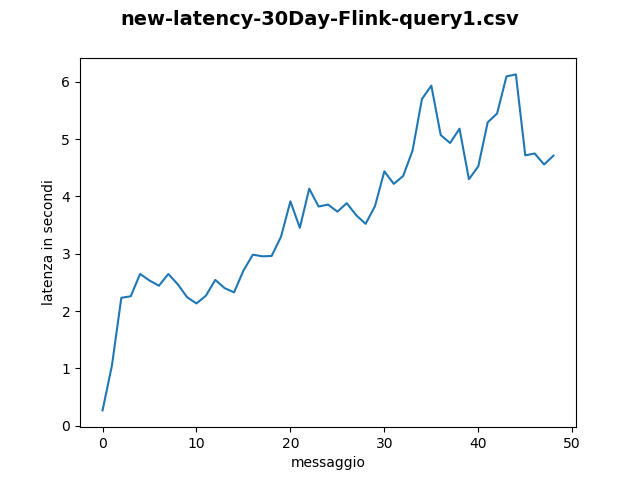
\includegraphics[width=14cm]{../results/tempi/new-latency-30Day-Flink-query1.csv.png}


\subsection{Kafka Streams}
ho trovato Kafka Stream a livello di sviluppo più difficoltoso inoltre dai test effettuati non è riuscito a "rimanere dietro" allo stremming dei dati tantè che mediamente aveva una latenza superiore ai due minuti.
Inoltre ho notato che kafka e flink hanno una gestione diversa delle finestre, flink non processa la finestra fino a quando non viene superato l'event time di fine finestra,mentre kafka appena arriva un nuovo record processa tutta finestra e se arriva un novo record che rientra ancora nella stessa finestra la riprocessa, questo potrebbe essere un motivo per la  differenza delle performance dei due framework.
Una cosa interessante è osservare il grafico della latenza di kafka stream
notiamo che la latenza arriva fino a un picco di oltre 200 secondi per poi iniziare a diminuire 
questo pattern è stato osservato in tutti i test fatti con kafka streams
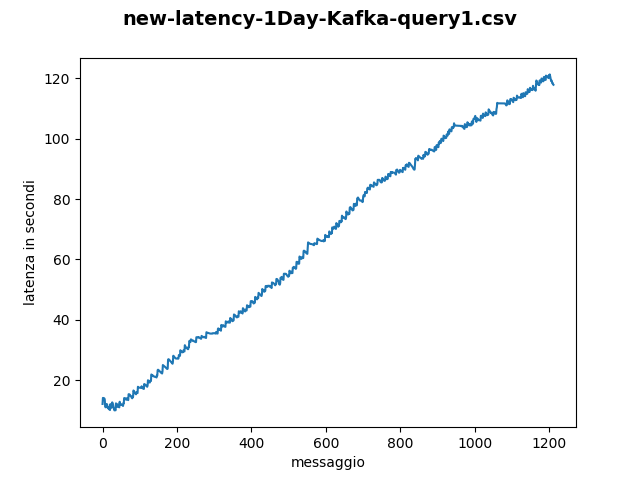
\includegraphics[width=14cm]{../results/tempi/new-latency-1Day-Kafka-query1.csv.png}

 





\end{document}
\endinput
%%
%% End of file `sample-acmsmall.tex'.
